\chapter{Electrochemical Energy Storage in Redox Conductive Polymers}
This chapter introduces chemical structures of organic electrode materials and discusses their electrochemical performance. The concept of organic radical battery is discussed, necessary electrochemical characterization and polymerization techniques are described. Preparation of electrochemically active organic cathode films is described, preparation of spectroscopic samples is described.

\section{Rechargeable Electrochemical Cells}

Two opposite electric charges separated from each other can store energy in an electrostatic field. It is possible to accumulate many charges on the plates of a capacitor and store some energy~\cite{He_2022}, but due to the technological difficulties, electrochemical cells are commonly used instead~\cite{Figgener_2020}. An electrochemical cell is an energy storage device and a power source that undergoes a chemical reaction to transfer some electric charge from one of its components to another through an external circuit. 

\begin{figure}[h]
\center
	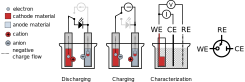
\includegraphics[width=0.75\textwidth]{./electrochemistry/figures/echem_cells.pdf}
	\caption{Rechargeable electrochemical cell with the electrical diagram for charging and discharging. Redox processes on the electrodes during charging and discharging. Three-electrode electrochemical cell used for electrochemical characterization of the electrodes.}
	\label{fig:echem_cells}
\end{figure}



A simple electrochemical cell consists of three elements: two spatially separated materials called electrodes, and a solution of mobile ions between them called electrolyte. The two electrodes have different work functions, or, chemically speaking, reduction-oxidation (redox) potentials. The potential difference between the two electrodes is called the open-circuit potential of the cell. When the electrodes are connected through an external circuit, as shown in Figure~\ref{fig:echem_cells}~a), the charge flows from one electrode to another through the circuit and the ions in the electrolyte rearrange to maintain charge balance~\cite{muench2016_chemrev}. While the cell delivers the electric current to the circuit, a chemical reaction is happening on its electrodes: the positively charged electrode, called cathode, is being reduced, obtaining electrons from the negatively charged anode through the external circuit. At the same time, the anode loses electrons and is being oxidized. If the electrodes can undergo a reversible redox reaction, a current applied to the cell restores its charged state, as shown in Figure~\ref{fig:echem_cells}~b).\\
The electrode of an organic electrochemical cell is made of a non-redox-active (metallic) lead and a layer of redox active (organic) molecules. The charge transfer between the conductor and the redox active molecule at the cell cathode can be described in terms of the energies of molecular orbitals of the cathode molecule~\cite{DOM}. When the electric potential $V$ of the biased metallic lead is set higher than the energy of the lowest unoccupied molecular orbital (LUMO) of the cathode molecule, an electron is transferred from the lead to the cathode molecule and the energy of the cathode molecule is increased to LUMO - the cathode molecule is reduced. If the lead is connected to the opposite electrode of the cell (through the external circuit), the electron transfer will decrease the When the electric potential of the lead is set below the ...\\


The speed, reversibility, released by-products and physical conditions of this redox reaction are the key factors that define the charging rate, cycling stability, the self-discharge rate and the area of application of an electrochemical cell. This type of redox reaction had been of great interest for the field of energy storage, particularly, electrochemistry, where numerous characterization techniques have been developed to optimize the architecture of electrochemical power sources. Depending on the redox potentials of the used electrodes, the output voltage of a cell ranges between 0 and 5~V. Most applications require higher voltages, so multiple cells are connected in series to form a battery.\\



State of charge (SoC).\\
State of health (SoH).\\
Gravimetric capacity.\\


DOM:\\
A conventional electrochemical cell requires at least two electrodes and one electrolyte.
While the electrodes provide electric conductivity, the electrolyte governs a conduc-
6tivity across the solvent, in most cases by mobile ions. Through applying an electric
potential between the electrode, a chemical reaction can occur in the electrolyte by
transferring electrons to or from the electrode. The driving force for this reaction is
the potential difference between the electrode and the analyte. The inherent so called
open-circuit potential of this cell, when no current is flowing is depending on the mate-
rials used in the cell, considering the electrodes as well as the redox-active material at
the electrodes. The charge transfer happening between electrode and active molecule,
can be explained by the potential in relation to the energy of the charge carries. If the
energy of the electrons on the electrode is higher than the lowest unoccupied molecular
orbital (LUMO), the electron is transferred to the active species leading to a reduction
current. In the other direction, if the electrode potential is lower than the highest occu-
pied molecular orbital (HOMO), the species transfers an electron to the electrode and
an oxidation current flows. For a reversible process, the potential associated with this
charge transfer is called standard potential of the reaction. The energy configuration
of the active species can be described by the Nernst equation.
This principle holds true for electrodes that contain multiple materials or adsorbed
redox-active species, since the processes of interest happen at the interfaces between
the species and phases. As convention the cell can be defined in the following notation
Au$/$PTMA, PTMA+ $/$(BF4)- , (Et4N)+ $/$AgCl$/$Ag
where the $/$ symbolizes a phase boundary and a , means that the species are present
in the same phase [19].
In many cases, the focus of the experiment lies on only one electrode which is therefore
identified as the working electrode (WE). The counterpart of this electrode is the
reference electrode (RE). Since the applied potential is measured against this reference
electrode, the standard potential a the RE has to be unaffected by the current flow.
This means, it should not undergo a chemical reaction and the chemical environment
should not change during the experiment. A general reference electrode is the standard
hydrogen electrode (P t/H2 /H + ) or SHE. The main difference between the various
references is their operation range and a constant potential shift with respect to the
SHE due to different equilibrium potentials. The used couple Ag/Ag + exhibits a shift
of 0.7991 V vs. SHE and for Ag/AgCl the shift is 0.2223 V against SHE [19], although
these values can only be used if the configuration is strictly equivalent to the one used
for determining them. In other cases the exact shifts might differ. A general scheme
of an electrochemical cell is shown in figure



\section{Electrochemical Instrumentation}
\subsection{Cyclic Voltammogram}
electrochemical setup. beaker, we ce re. electrolyte. cycling limits and rate. redox peaks. quantitative cv.
\subsection{Charge-Discharge Cycling}
\label{sec:echem_charging}
galvanostatic and potentiostatic cycling. measuring cell capacity.

\section{Redox Conductive Polymers}

Redox active macromolecules or polymers~\cite{Staudinger_1920} are known since 1940s due to the works of Lauth~\cite{Lauth_1944} and Cassidy~\cite{Cassidy_1949} on electron exchange polymers. After the discovery of the conductivity of polyacetylene by Shirakawa, Heeger and McDiarmid in 1977~\cite{Shirakawa_1977}, polymers with sufficient charge transport were synthesized~\cite{} and the field of organic electronics had emerged and expanded. 

\par

The key for polymer conductivity is the p $\pi$ - conjugated network, a system of overlapping $\pi$ orbitals of carbon in a chain of alternating single and double carbon-carbon bonds that allows charge delocalization along the polymer backbone. An example of a $\pi$ conjugated network is polyacetylene. Polyacetylene exhibits a band structure in the electron energy levels (between $\pi$ and $\pi^\star$ orbitals) and represents a molecular semiconductor.

\par

Organic solar cells~\cite{Lee_1993} and organic field effect transistors~\cite{Koezuka_1987} contain conjugated polymers that have electrical properties of semiconductors, yet can be easily printed in form of thin flexible films without using high temperatures. Combining the conductive polymers with stable radical side groups has formed the class of redox conductive polymers and lead to the concept of an organic radical battery~\cite{Rohland_2021}.




\section{Organic Radical Battery}

Batteries based on conjugated polymers containing stable radical moieties as high-capacitance groups represent a promising class of future electrochemical power sources - organic radical batteries (ORB)~\cite{nakahara2002_cpl, nishide2004_electact,xie2021_mathoriz,Rohland2022}. ORB combine the advantages of high-power supercapacitors, namely high discharge rates, and the high energy density of conventional lithium-ion technology. In contrast to the lithium-ion battery, the charging of an organic battery does not involve intercalation of metal ions into the electrodes. This reduces the structural change of the electrode upon repeated recharging which allows for a longer cycle life of an ORB. The semi-conducting nature of organic electrodes reduces the Joule heating during the battery operation, and this allows for higher charge/discharge rates. The amorphous and swollen structure of organic electrodes allows the electrolyte ions to diffuse faster into the electrode, which also increases the charge/discharge rate~\cite{nishide_2009}. A further beneficial property of organic materials over traditional inorganic materials is their availability and the low cost of the starting materials for the synthesis of the target polymers in conjunction with good mechanical properties~\cite{janoschka2012_advmater, muench2016_chemrev, friebe2017_topcurrchem}. The large knowledge base on polymer processing allows for inkjet printing, roll-to-roll processing and other low-cost manufacturing techniques for making low-cost, flexible and light-weight integrated devices, including flexible plastic batteries~\cite{janoschka2012_advmater,nishide_2009}. 

\section{Organic Electrode Materials}
ORB based on redox polymers containing stable radicals~\cite{nakahara2002_cpl} have been shown to compete with or even outperform  conventional Li based batteries in terms of power densities~\cite{IWASA2007} with the additional benefit of being free from rare precursors, inheriting mechanical properties of plastics and electrical properties of semiconductors~\cite{friebe2017_topcurrchem,Casado2021,Goujon2021}. Advanced molecular design techniques allow for tuning of the electrochemical properties of the redox polymers~\cite{Janoschka2017}, that brings in a rich variety of organic energy storage materials~\cite{Xie2021,Vereshchagin2022,Janoschka2017a} and creates a large room for their optimization. 

\par
\subsection{TEMPO}
TEMPO (2,2,6,6-tetramethylpiperidine-1-oxyl) shown in Figure~\ref{fig:molecules}~a) is a small molecule and a stable radical that can undergo a fast and reversible redox reaction between TEMPO$^\bullet$ and TEMPO$^+$. TEMPO is an inexpensive organic compound~\cite{Vereshchagin2022} produced from acetone with liquid ammonia, hydrazine and peroxide~\cite{Casado_2021_book}. TEMPO radicals are widely used as spin labels studies of biological systems with electron spin resonance~\cite{emagres}, because the unpaired electron of TEMPO$^\bullet$ has a well defined spectral signature that changes when the local environment of a TEMPO fragment changes.

TEMPOL is a TEMPO with an OH group. It forms crystals.

\begin{figure}[h]
\center
	
\includegraphics[width=1\textwidth]{./electrochemistry/figures/materials/molecules.pdf}
	\caption{Chemical structures of the molecular fragments and polymers that were used for making a battery cathode containing stable nitroxide radicals.}
	\label{fig:molecules}
\end{figure}



Redox conductive conjugated polymers containing TEMPO redox groups, as pDiTBuS (poly-di-TEMPO-Butyl-Salen) shown in Figure~\ref{fig:Figure_1}, demonstrate particularly promising energy and power densities~\cite{Vereshchagin2020}. The pDiTBuS was designed as a cathode material: it is oxidized when the electrochemical cell containing this material is charged. A film of pDiTBuS comprises a high concentration of redox active stable nitroxyl radicals attached to a conjugated polymer backbone that interconnects them as a molecular wire. Such system can be viewed as a highly disordered molecular hole-transporting semiconductor (the poly-NiSalen backbone) that contains a large amount of hole traps (TEMPO groups) attached to it with butyl linkers. When the film is reduced (discharged), the TEMPO groups are in the radical state and act as unfilled traps. Upon oxidation (charging), the TEMPO fragments lose an unpaired electron and acquire a positive charge, so the traps are being filled with holes. The reversible redox reaction in the pDiTBuS film is demonstrated in a cyclic \ik{voltammogram} shown in Figure~\ref{fig:Figure_S1} (see ESI).

\par
While active electrode materials with nitroxide radicals as redox-active groups are ideally suited for organic radical batteries (ORBs) that exhibit high power densities, the broad application of most nitroxide-based materials is limited by their moderate electrical properties. A promising route towards overcoming the conductivity problem is the use of polymers that combine radical-containing moieties and a conductive backbone. This strategy was successfully followed in a number of studies focusing on different polymers.\cite{oyaizu2015_polymerjournal, bahaceci2013_jpowersources, katsumata2006_mrc, xu2014_electact, aydin2015_jsoistatelect, schwartz2018_synthmet}

\par

The flexible molecular design together with questions regarding unresolved charge transport- and performance limiting mechanisms have inspired a variety of characterization techniques to be developed and applied to both energy storage materials and energy storage devices, operando and ex-situ. Together with electrochemical characterization as the standard method for studying the properties of energy storage materials\cite{IWASA2007,Zens2022}, operando optical microscopy~\cite{Merryweather2022}, neutron imaging~\cite{Ma2020} and X-ray diffraction~\cite{Rhodes2012} were applied to monitor irreversible structural deformations during extreme charging of Li cells.

\subsection{PTMA}

A simple organic radical polymer containing TEMPO is poly(2,2,6,6-tetramethyl-1-piperidinyloxy-4-yl methacrylate) (PTMA, Figure~\ref{fig:molecules}~c). The polymer backbone of PTMA consists of single C-C bonds and therefore is not conductive, so the transport of charge in a PTMA film has to be mediated by adding conductive mesh such as activated carbon. When mixed with conductive carbon additive, PTMA has become a standard cathode material for ORBs and Li-ORBs, providing a discharge cell voltage of 3.5~V (with a Li anode) and a theoretical discharge capacity of $C_{theo}=111$~mAh/g~\cite{Daniel2023_Multimodal}. PTMA is soluble in acetonitrile (AN), chloroform (CF), tetrahydrofurane and dichlormethane. It is claimed to be insoluble in toluene, ethers, carbonates, and alcohols, however it becomes gel-like with some of these solvents~\cite{DOM}.

\subsection{NiSalen}
The molecular backbone of a redox conductive polymer has to conduct electric charge. A NiSalen molecule is a Schiff complex of Ni that has a conjugated path through it. The conductivity of NiSalen was measured. Upon oxidation of a polymeric NiSalen, the formation of positive polarons was observed in it with UV-Vis spectroscopy~\cite{Timonov}, that suggests p-NiSalen is a p-type molecular semiconductor. p-NiSalen exhibits electrochemical capacity and can store up to two positive charges per monomer unit.


\subsection{pDiTBuS}
Redox conductive conjugated polymers containing TEMPO (2,2,6,6-tetramethylpiperidine-1-oxyl) redox groups, as pDiTBuS (poly-di-TEMPO-Butyl-Salen) shown in Figure~\ref{fig:Figure_1}, demonstrate particularly promising energy and power densities~\cite{Vereshchagin2020}. The pDiTBuS was designed as a cathode material: it is oxidized when the electrochemical cell containing this material is charged. A film of pDiTBuS comprises a high concentration of redox active stable nitroxyl radicals attached to a conjugated polymer backbone that interconnects them as a molecular wire. Such system may be viewed as a highly disordered molecular hole-transporting semiconductor (the poly-NiSalen backbone) that contains a large amount of hole traps (TEMPO groups) attached to it with butyl linkers. When the film is reduced (discharged), the TEMPO groups are in the radical state and act as unfilled traps. Upon oxidation (charging), the TEMPO fragments lose an unpaired electron and acquire a positive charge, so the traps are being filled with holes.

\begin{figure}[h]
\center
	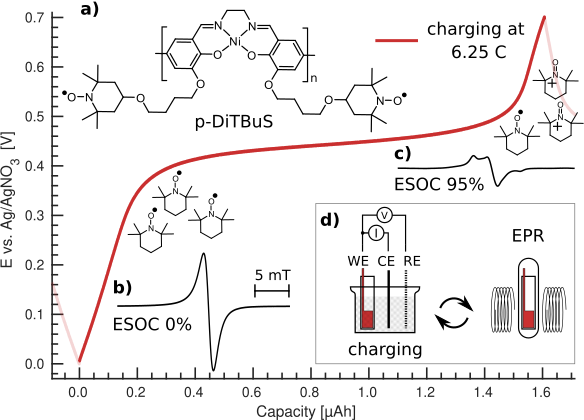
\includegraphics[width=0.7\textwidth]{./introduction/figures/Figure_1.pdf}
	\caption{Galvanostatic charge-discharge curve for a pDiTBuS cathode film at 10~$\muup$A (6.25~C), chemical structure of pDiTBuS (a), normalized cwEPR spectral signatures for reduced (b) and oxidized (c) states. Scheme of the ex-situ EPR measurement on the pDiTBuS half cell (d).}
	\label{fig:Figure_1}
\end{figure}

\subsection{pDiTS}


\subsection{Electro-polymerization of TEMPO-Salens}
The process of polymerization is connecting multiple monomer units of one sort to a continuous molecular chain. Among various polymerization techniques, redox conductive molecules with pendant charge bearing groups the cyclic electropolymerization turned out to be an efficient technique. \\
Fast And Capacious:\\
"Electrochemical polymerization of DiTS was studied by means of the EQCM technique on piezoelectric crystals coated with platinum using a linear voltage sweep. The CV of DiTS (Figure FAC2A) shows the paired peaks A and A' at 0.55 V and 0.47 V respectively, which correspond to charging and discharging of the nitroxyl fragments. An irreversible anodic peak B corresponds to oxidative coupling of the NiSalen fragments
of DiTS, which results in the polymer p-DiTS~\cite{Vereshchagin_2019,Koshika_2009}. The gradual
increase of the CV current and the electrode mass (Figure FAC2A) in the subsequent cycles indicates the course of the polymerization process. An unusual feature in the EQCM curves, recorded during the electropolymerization process, is that the mass growth at the electrode occurs predominantly at potentials below the peak A' (Figure FAC2A), which is in contradiction to previous reports on the deposition of a NiSalen-type polymer, where polymerization occurs at potentials above the oxidation peak of the monomeric NiSalen.[22]
The CV sweep boundaries were varied to establish the optimal conditions for the polymerization of DiTS. Only the
redox peaks of the TEMPO moieties in solution are observed on CV (Figure 2C, curve i) while sweeping in 0.40–0.75 V range without polymer formation. An extension of the anodic
boundary to 0.90 V (Figure FAC2C, curve ii) led to an increase in EQCM mass and CV current, which indicates the polymer growth on the electrode surface. Further extension of the anodic region of the CV range (Figure 2C, curve iv) did not improve the polymerization process, but led to a decrease of
the conductivity of the film due to overoxidation (Figure FACS4), highlighting 0.90 V as an optimal position of the anodic boundary. While polymerization is possible at higher potentials on the surface of a clean substrate, low conductivity of the overoxidized film is blocking further monomer oxidation on the
surface, leading to rapid decrease in monomer oxidation current (Figure S4 and Figure 2C, curve iv). When the cathodic boundary was set near the A/A’ pair and the CV was performed
between 0.35 V and 0.90 V (Figure FAC2C, curve iii), no polymerization occurred, emphasizing the crucial role of the charge-discharge of the nitroxyl fragments in the polymerization process.\\

The conventional mechanism for the chain growth of polymeric NiSalens is based on the formation of radical cation
species. Although the NiSalen-centered radical cations of DiTS
are formed on the peak B (Figure FAC2A), apparently the polymerization proceeds at a low rate in this area of potentials, compared to other NiSalen type complexes~\cite{Novozhilova_2009}. Based on the
obtained results, we assume that the positive charge density both on the monomer molecules and deposited polymer layers grow rapidly above the A (Figure FAC2A) peak potential due to simultaneous oxidation of the NiSalen core and two TEMPO fragments in one molecule. High charge density causes intermolecular coulombic repulsion, acting as a coulombic "shield", which hinders the coupling of radical cation species and prevents the chain growth. As soon as the potential has decreased to the A' (Figure FAC2A) peak on the negative scan of the CV (Figure S5C, point C), rapid polymer growth occurred due to the discharge of the p-DiTS film, which deactivates the
coulombic shield. The formation of the polymer proceeds until the shield recovers during the next CV cycle due to the oxidation of nitroxyl fragments. At this point, a sharp decrease in mass occurs due to the desorption of the monomeric DiTS molecules repelled by the charging coulombic shield. The scheme of this process is depicted in Figure FAC2B and a scheme of the polymer formation process in Figure FAC2D.\\ 

The mass growth for one deposition cycle is ca. 0.3 ug cm 2 both for 5 mV s 1 and 50 mV s 1 CVs. Polymer deposition is observed both at potentials higher than 0.8 V and lower than 0.4 V, and during low rate CV almost two thirds of the overall polymer mass is formed at potentials more positive than the potentials of the
A/A' peaks. On the contrary, at 50 mV/s only one third of the polymer is formed at potentials higher than 0.8 V. This indicates that the Coulombic shielding from oxidized TEMPO groups allows coupling between the radical cations of DiTS and the charged TEMPO groups, though at quite low rate. The
possibility of polymerization at both potential regions was confirmed by the experiment consisting of a series of
successive iterations of potentiostatic and potentiodynamic syntheses, as well as open-circuit rest periods (See SI and Figure FACS6 for further discussion)"

\begin{figure}[h]
\center
	\includegraphics[width=1\textwidth]{./electrochemistry/figures/DFT_DITS.pdf}
	\caption{Spin density in a single DiTS monomer unit for various oxidation states calculated by Marcel Gauglitz with density-functional theory in ORCA~\cite{ORCA} at the high-performance computing cluster of the Free University Berlin~\cite{HPC_FUB} using the def2-TZVP functional basis set. a): neutral DiTS with two radicals, b) singly oxidized DiTS (one hole injected), b) doubly oxidized DiTS showing no spin density, c) DiTS$^{3+}$ showing a positive polaron localized on the NiSalen backbone, d) DiTS$^{4+}$ showing increased spin density on the backbone.}
	\label{fig:DiTS_DFT}
\end{figure}



\subsection{Charge Transport Model for Redox Conductive Polymers}
A transfer of charge in a highly disordered molecular system, such as a film of a conjugated polymer, can be described in terms of hopping of charge carriers between the intertwined polymer fragments under external electric field. The molecular systems for electrochemical charge storage are inherently disordered materials and the electric performance of a film containing those molecules is is strongly dependent on the deposition method, as well as on the molecular structure See \cite{Xie2021} (!). Therefore, so far there has not been a unified physical model that would describe the charge transport phenomena in such materials. The particular charge transport models have been developed that are applicable to certain classes of polymers (read that chapter in the polymer book and show what was done).

